\paragraph{QuizziPedia::Front-End::Views::TrainingView}
\begin{figure} [ht]
	\centering
	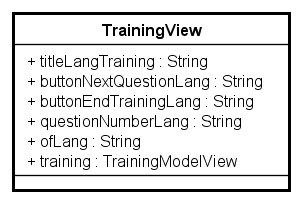
\includegraphics[scale=0.80]{UML/Classi/Front-End/QuizziPedia_Front-end_Views_TrainingView.png}
	\caption{QuizziPedia::Front-End::Views:TrainingView}
\end{figure} \FloatBarrier
\begin{itemize}
	\item \textbf{Descrizione}: \textit{view\ped{G}} principale della modalità allenamento; conterrà i vari templates di ogni domanda dell'allenamento;
	\item \textbf{Utilizzo}: all'interno di essa verrà caricato inizialmente il template dove si potranno scegliere l'argomento e le parole chiave dell'allenamento; verranno poi caricati i templates di ogni domanda in base alle preferenze scelte; 
	\item \textbf{Relazioni con altre classi}:
	\begin{itemize}
		\item \textbf{IN \texttt{TrainingModelView}}: classe di tipo modelview la cui istanziazione è contenuta all'interno della variabile di ambiente \texttt{\$scope} di \textit{Angular\ped{G}}. All'interno di essa sono presenti le variabili e i metodi necessari per il \textit{Two-Way Data-Binding\ped{G}} tra la \textit{view\ped{G}} \texttt{TrainingView} e il \textit{controller\ped{G}} \texttt{TrainingController};
		\item \textbf{IN \texttt{QuestionsModelView}}: classe di tipo modelview la cui istanziazione è contenuta all'interno della variabile di ambiente \texttt{\$scope} di \textit{Angular\ped{G}}. All'interno di essa sono presenti le variabili e i metodi necessari per il \textit{Two-Way Data-Binding\ped{G}} tra le \textit{directive\ped{G}} che compongono dinamicamente la vista della domanda e il \textit{controller\ped{G}} \texttt{QuestionsController};
		\item \textbf{IN \texttt{TrainingSetUpDirective}}: rappresenta il componente grafico che permette all'utente di selezionare l'argomento e le parole chiave per iniziare un allenamento con queste caratteristiche. Viene visualizzato	dinamicamente all'interno delle \textit{views\ped{G}} \texttt{TrainingView} e \texttt{FillingQuestionnaireView} mediante il \textit{controller\ped{G}} \\\texttt{QuestionsController};
		\item \textbf{IN \texttt{HeaderTextQuestionDirective}}:rappresenta il componente grafico che presenta all'utente il testo della domanda, l'argomento e le parole chiave. Viene visualizzato dinamicamente all'interno delle \textit{views\ped{G}} \texttt{TrainingView} e \texttt{FillingQuestionnaireView} mediante il \textit{controller\ped{G}} \texttt{QuestionsController};
		\item \textbf{IN \texttt{TrueFalseAnswerDirective}}: rappresenta il componente grafico che permette all'utente di visualizzare la domanda vero e falso. Viene visualizzato dinamicamente all'interno delle \textit{views\ped{G}} \texttt{TrainingView} e \texttt{FillingQuestionnaireView} mediante il \textit{controller\ped{G}} \texttt{QuestionsController};
		\item \textbf{IN \texttt{MultipleChoiceAnswerDirective}}: rappresenta il componente grafico che permette all'utente di visualizzare la domanda a risposta multipla. Viene visualizzato dinamicamente all'interno delle \textit{views\ped{G}} \texttt{TrainingView} e \texttt{FillingQuestionnaireView} mediante il \textit{controller\ped{G}} \texttt{QuestionsController};
		\item \textbf{IN \texttt{LinkingAnswerDirective}}: rappresenta il componente grafico che permette all'utente di visualizzare la domanda di collegamento. Viene visualizzato dinamicamente all'interno delle \textit{views\ped{G}} \texttt{TrainingView} e \texttt{FillingQuestionnaireView} mediante il \textit{controller\ped{G}} \texttt{QuestionsController};
		\item \textbf{IN \texttt{SortImagesAnswerDirective}}: rappresenta il componente grafico che permette all'utente di visualizzare la domanda ad ordinamento di immagini. Viene visualizzato dinamicamente all'interno delle \textit{views\ped{G}} \texttt{TrainingView} e \texttt{FillingQuestionnaireView} mediante il \textit{controller\ped{G}} \texttt{QuestionsController};
		\item \textbf{IN \texttt{SortTextAnswerDirective}}: rappresenta il componente grafico che permette all'utente di visualizzare la domanda ad ordinamento di stringhe. Viene visualizzato dinamicamente all'interno delle \textit{views\ped{G}} \texttt{TrainingView} e \texttt{FillingQuestionnaireView} mediante il \textit{controller\ped{G}} \texttt{QuestionsController};
		\item \textbf{IN \texttt{EmptySpaceAnswerDirective}}: rappresenta il componente grafico che permette all'utente di visualizzare l'esercizio a riempimento di spazi vuoti. Viene visualizzato dinamicamente all'interno delle \textit{views\ped{G}} \texttt{TrainingView} e \texttt{FillingQuestionnaireView} mediante il \textit{controller\ped{G}} \texttt{QuestionsController};
		\item \textbf{IN \texttt{ClickableAnswerDirective}}: rappresenta il componente grafico che permette all'utente di visualizzare la domanda ad area cliccabile nell'immagine. Viene visualizzato dinamicamente all'interno delle \textit{views\ped{G}} \texttt{TrainingView} e \texttt{FillingQuestionnaireView} mediante il \textit{controller\ped{G}} \texttt{QuestionsController};
		\item \textbf{IN \texttt{LangModel}}: rappresenta il modello delle informazioni per la giusta traduzione dell'applicazione.
	\end{itemize}
	\item \textbf{Attributi}:
	\begin{itemize}
		\item \texttt{+ titleLangTraining: String} \\ Attributo che viene utilizzato per visualizzare la giusta traduzione del titolo della pagina, in italiano o in inglese;
		\item \texttt{+ questionNumberLang: String} \\ Attributo che viene utilizzato per visualizzare la giusta traduzione della frase "domanda numero";
		\item \texttt{+ ofLang: String} \\ Attributo che viene utilizzato per visualizzare la giusta traduzione della parola "di";
		\item \texttt{+ buttonNextQuestionLang: String} \\ Attributo che viene utilizzato per visualizzare la giusta traduzione della \textit{label\ped{G}} per il bottone di avanzamento a domanda successiva, in italiano o in inglese;
		\item \texttt{+ buttonEndTrainingLang: String} \\ Attributo che viene utilizzato per visualizzare la giusta traduzione della \textit{label\ped{G}} per il bottone di conclusione dell'allenamento, in italiano o in inglese;
		\item \texttt{+ training: TrainingModelView} \\ Oggetto di tipo \texttt{TrainingModelView}, popolato solamente dopo aver iniziato l'allenamento, contenente al suo interno i seguenti campi:
		\begin{itemize}
			\item \texttt{+ argument: String} \\ Attributo che rappresenta l'argomento scelto;
			\item \texttt{+ keywords: Array[String]} \\ \texttt{array} di stringhe che contiene le parole chiave scelte;
			\item \texttt{+ questionNumber: String} \\ Attributo che rappresenta il numero progressivo della domanda attuale;
			\item \texttt{+ numberOfQuestions: String} \\ Attributo che rappresenta il numero di domande scelte.
		\end{itemize}
	\end{itemize}
\end{itemize}